\newcommand\PCOS[1]{\footnotesize obs.\ref{#1}: {\nameref{#1}}}
\newcommand\PCIS[1]{\footnotesize int.\ref{#1}: {\nameref{#1}}}

% Please add the following required packages to your document preamble:
% \usepackage[normalem]{ulem}
% \useunder{\uline}{\ul}{}

\begin{figure}[htp]
    \centering
    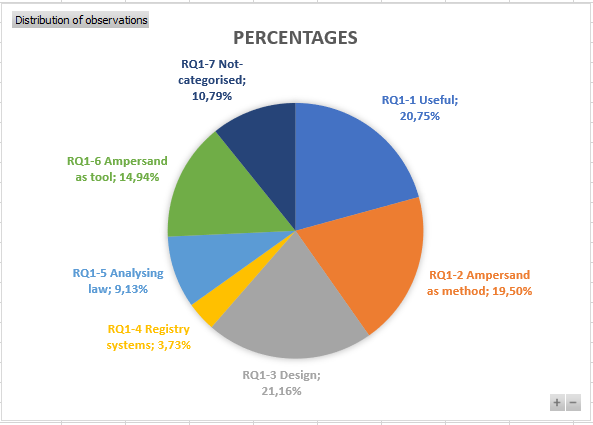
\includegraphics[width=0.7\textwidth]{docs/AF-SE/00_common/04_images/content_analysis.PNG}
    \caption{Content observations Distribution}
    \label{fig:content distribution}
\end{figure}

\def\head{\textbf{RQ1-1, Category:Useful, Reference to observation/interview}}
\begin{xltabular}{\textwidth}{|X|}
\caption{List of observations \head} \\ \hline 
\multicolumn{1}{|l|}{\head}  \\ \hline 
\endfirsthead
{{\bfseries \tablename\ \thetable{} -- continued from previous page}} \\
\hline 
\multicolumn{1}{|l|}{\head}  \\ \hline 
\endhead
\hline \multicolumn{1}{|r|}{{Continued on next page}} \\ \hline
\endfoot \hline \hline
\endlastfoot

\PCIS{int:I-4.5}\\
\PCOS{obs:rq1-11}\\
\PCOS{obs:rq1-18}\\
\PCOS{obs:rq1-13:17-10}\\
\PCOS{obs:rq1-36:29-9}\\
\PCOS{obs:rq1-47:27-10}\\
\PCOS{obs:rq1-6:21-10}\\
\PCOS{obs:rq4-8:22-11}\\

\PCOS{obs:rq1-17}\\
\PCOS{obs:rq1-60:9-11}\\
\PCOS{obs:rq1-96:30-12}\\

\PCIS{int:I-3.7}\\
\PCOS{obs:rq1-2}\\
\PCOS{obs:rq1-25:12-9}\\
\PCOS{obs:rq1-31:14-9}\\

\PCOS{obs:rq1-42:19-10}\\
\PCOS{obs:rq1-45:24-10}\\
\PCOS{obs:rq1-46:24-10}\\
\PCOS{obs:rq1-97:30-12}\\

\PCIS{int:I-3.2}\\
\PCOS{obs:rq3-7}\\

\PCOS{obs:rq1-42:21-10}\\

\PCIS{int:I-1.3}\\
\PCIS{int:I-1.8}\\
\PCIS{int:I-2.10}\\
\PCOS{obs:rq1-62:10-11}\\

\PCIS{int:I-2.2}\\
\PCOS{obs:rq4-2}\\
\PCOS{obs:rq4-5}\\
\PCOS{obs:rq1-70:14-11}\\
\PCOS{obs:rq1-72:14-11}\\
\PCOS{obs:rq1-73:14-11}\\
\PCOS{obs:rq1-74:16-11}\\
\PCOS{obs:rq1-8:14-11}\\

\PCIS{int:I-2.5}\\
\PCIS{int:I-4.8}\\
\PCOS{obs:rq4-7}\\
\PCOS{obs:rq1-63:10-11}\\

\PCIS{int:I-4.6}\\
\PCOS{obs:rq2-18:16-11}\\

\PCIS{int:I-1.2}\\
\PCIS{int:I-1.6}\\

\PCIS{int:I-4.11}\\
\PCIS{int:I-4.12}\\
\PCIS{int:I-4.3}\\
\PCIS{int:I-4.9}\\
\PCOS{obs:rq1-39:3-10}\\
\PCOS{obs:rq1-7:10-11}\\
\PCOS{obs:rq2-16:19-10}\\
\PCOS{obs:rq3-16:24-10}\\


%-	rq1-11 Implementation in Docker with RAP creates new directories all the time.
%\\-	rq1-13:17-10: The setup of Ampersand in local environment is specific and not self-explanatory.
%\\-	rq1-17 Applying a rule requires a lot of patience and practice.
%\\-	rq1-18 Can not find an example on the internet, only in the repo of Ampersand itself.
%\\-	rq1-39:3-10: Do not forget to create delete rules in addition to append and edit rules in the {rule}\textbf{s} in the context of the \A{Lifecycle} approach.
%\\-	rq1-42:19-10: Immediately add the description when recording a {concept} and \A{relation}.
%\\-	rq1-42:21-10: It is easy to deviate from the legal texts.
%\\-	rq1-45:24-10: Overview within a Ampersandscript is difficult to maintain and obtain.
%\\-	rq1-46:24-10: There is no find able relationship between the \A{relation} and the {concept} in the script.
%\\-	rq1-47:27-10: Detecting a bug.
%\-	rq1-60:9-11: The process of writing a \A{Ampersand} script is not without practice.
%\-	rq1-62:10-11: There has be the \A{architecture} link between the {law core} and the {register core}
%\-	rq1-63:10-11: Ampersand is \A{flexible} by extension concepts and relationships.
%\\-	rq1-7:10-11: Each \A{relation} is part of a record structure.
%\\-	rq1-70:14-11: Postman works with api/v1/resource, e.g. GET \url{localhost/api/v1/resource/Person/P001/Person}, retrieves that of an existing person.
%\\-	rq1-73:14-11: Ampersand can be used from other applications through \A{api}'s, but the return values are next to the requested information also messages and not message codes.
%\\-	rq1-96:30-12: Skill in scripting within \A{Ampersand} is quickly lost if you don't do this frequently.
%\\-	rq1-97:30-12: By puzzling with Ampersand people quickly forget to make correct \A{documentation}.
%\\-	rq2-12:19-10: TOT has the property that this must be entered in the \A{interface} because otherwise the data will not be saved.
%\\-	rq2-16:19-10/11-11: Ampersand has a hard time determining a period.
%\\-	rq2-18:16-11: Good to realize that the {meaning} you write down also ends up in the \A{Conceptual analysis}.
%\\-	rq3-7 Adding \A{documentation} with the correct description to a concept and relation is not so easy.
%\\-	rq4-5 Postman used for \A{api} link with Ampersand.
%\\-	rq4-7 What happens if \A{Ampersand} is implemented and there are changes in the structure (normal for software)
%\\-	rq4-8:22-11: The team behind \A{Ampersand} is very dedicated.
%\\-	 rq1-8:14-11: No swagger is created for the \A{api}
%\\-	rq1-46:24-10: There is no find able relationship between the {relation} and the \A{concept} in the script.
%\\-	 rq1-6:21-10/30-10: \A{Docker} is also another thing to learn.
%\\-	 rq1-17 Applying a \A{rule}\textbf{s} takes a lot of patience and practice.
%\\-	 rq2-4:30-9: Which agreements must be made regarding the structure of the descriptions for \A{Conceptual analysis}.
%\\-	 rq3-16:24-10: For the Netherlands, we have a country table from the RvIG.
%\\-	 rq4-2 The \A{api} link works fine, but entire messages return.
%\\-	Ampersand can be interesting, because it will be able to clear conflicting matters from the law.
%\\-	The registry core, an architecture model of CIBG, uses shared concepts
%\\-	In addition, the implementation must be such that the effective dates of the specific amendments to the law are also taken into account.
%\\-	Ampersand's possible positioning is to use it as an interpreter of legislation and regulations
%\\-	Ampersand has APIs and that is interesting to be able to link with
%\\-	When maintenance takes place on the model, how do we get from one model to another
%\\-	Ampersand's approach is in line with the \acrlong{rk}, but not at the implementation level.
%\\-	An addition of Ampersand is that a prototype is made that can also be tested. 
%\\-	A draft of the conceptual analysis is available and this is experienced as trusted by the lawyer. 
%\\-	Going through the law should be a first step for the conceptual analysis.
%\\-	The prototype shown is not easy for the user to understand.
%\\-	Ampersand's deployment could be applied to new tasks.
%\\-	For use, the question is how quickly a base is set up
%\\-	Ampersand method is a way of writing things down
%\\-	How is the maintenance of the system? A new model is always made with the help of Ampersand.
%\\-	The learning curve doesn't seem that big. 
%\\-	The question is whether the system will only work for simple registers or whether we can also use it to tackle complex registers.
%\\-	A follow-up study could be to make a comparison between a system built traditionally and a system built on the Ampersand method. 

\end{xltabular}


\def\head{\textbf{RQ1-2, Category:Ampersand as method, Reference to observation/interview}}
\begin{xltabular}{\textwidth}{|X|}
\caption{List of observations \head} \\ \hline 
\multicolumn{1}{|l|}{\head}  \\ \hline 
\endfirsthead
{{\bfseries \tablename\ \thetable{} -- continued from previous page}} \\
\hline 
\multicolumn{1}{|l|}{\head}  \\ \hline 
\endhead
\hline \multicolumn{1}{|r|}{{Continued on next page}} \\ \hline
\endfoot \hline \hline
\endlastfoot
\PCOS{obs:rq1-30:12-9}\\
\PCOS{obs:rq1-33:14-9}\\
\PCOS{obs:rq1-38:3-10}\\
\PCOS{obs:rq1-46:24-10}\\
\PCOS{obs:rq1-80:20-11}\\
\PCOS{obs:rq2-4:30-9}\\
\PCOS{obs:rq1-3}\\
\PCOS{obs:rq2-2}\\
\PCOS{obs:rq1-21:7-11}\\
\PCOS{obs:rq1-58:8-11}\\
\PCOS{obs:rq2-11:19-10}\\
\PCOS{obs:rq2-12:19-10}\\
\PCOS{obs:rq2-13:19-10}\\
\PCOS{obs:rq2-5:2-10}\\
\PCOS{obs:rq1-4}\\
\PCOS{obs:rq1-61:9-11}\\
\PCOS{obs:rq1-63:10-11}\\
\PCOS{obs:rq1-67:11-11}\\
\PCOS{obs:rq2-19:16-11}\\
\PCOS{obs:rq2-6:2-10}\\
\PCOS{obs:rq1-79:20-11}\\
\PCOS{obs:rq1-91:14-12}\\
\PCIS{int:I-1.4}\\
\PCIS{int:I-3.7}\\
\PCIS{int:I-4.13}\\
\PCOS{obs:rq1-42:19-10}\\
\PCOS{obs:rq1-51:2-11}\\
\PCOS{obs:rq1-84:30-11}\\
\PCIS{int:I-1.8}\\
\PCIS{int:I-2.11}\\
\PCIS{int:I-3.1}\\
\PCIS{int:I-3.2}\\
\PCIS{int:I-4.2}\\
\PCOS{obs:rq1-57-1:7-11}\\
\PCIS{int:I-1.1}\\
\PCIS{int:I-1.9}\\
\PCIS{int:I-4.10}\\
\PCIS{int:I-4.14}\\
\PCIS{int:I-4.5}\\
\PCIS{int:I-4.9}\\
\PCOS{obs:rq1-55:2-11}\\
\PCOS{obs:rq1-7:10-11}\\
\PCOS{obs:rq2-10:19-10}\\
\PCOS{obs:rq2-14:19-10}\\
\PCOS{obs:rq2-8:7-10}\\

\end{xltabular}


\def\head{\textbf{RQ1-3, Category:Design, Reference to observation/interview}}
\begin{xltabular}{\textwidth}{|X|}
\caption{List of observations \head} \\ \hline 
\multicolumn{1}{|l|}{\head}  \\ \hline 
\endfirsthead
{{\bfseries \tablename\ \thetable{} -- continued from previous page}} \\
\hline 
\multicolumn{1}{|l|}{\head}  \\ \hline 
\endhead
\hline \multicolumn{1}{|r|}{{Continued on next page}} \\ \hline
\endfoot \hline \hline
\endlastfoot
\PCIS{int:I-1.12}\\
\PCIS{int:I-1.3}\\
\PCIS{int:I-2.1}\\
\PCIS{int:I-2.6}\\
\PCIS{int:I-2.7}\\
\PCIS{int:I-2.8}\\
\PCOS{obs:rq4-1}\\
\PCOS{obs:rq4-3}\\
\PCOS{obs:rq1-63:10-11}\\
\PCOS{obs:rq1-89:7-12}\\

\PCOS{obs:rq1-1}\\
\PCOS{obs:rq1-75:20-11}\\
\PCOS{obs:rq1-78:20-11}\\
\PCOS{obs:rq1-99:6-1}\\
\PCOS{obs:rq2-18:16-11}\\

\PCOS{obs:rq1-39:3-10}\\
\PCOS{obs:rq1-95:29-12}\\

\PCOS{obs:rq1-92:14-12}\\
\PCOS{obs:rq1-93:19-12}\\
\PCOS{obs:rq3-8:19-9}\\

\PCIS{int:I-4.2}\\
\PCOS{obs:rq1-36:3-10}\\
\PCOS{obs:rq1-69:14-11}\\

\PCIS{int:I-4.7}\\
\PCOS{obs:rq2-17:10-11}\\
\PCOS{obs:rq3-10:12-10}\\
\PCOS{obs:rq3-11:12-10}\\

\PCOS{obs:rq1-71:14-11}\\

\PCIS{int:I-1.10}\\
\PCIS{int:I-3.4}\\
\PCIS{int:I-3.5}\\
\PCIS{int:I-4.8}\\

\PCIS{int:I-4.4}\\
\PCOS{obs:rq4-2}\\
\PCOS{obs:rq4-4}\\
\PCOS{obs:rq4-7}\\
\PCOS{obs:rq2-14:19-10}\\
\PCOS{obs:rq2-15:19-10}\\
\PCOS{obs:rq2-9:7-10}\\


\end{xltabular}

\def\head{\textbf{RQ1-4, Category:Registry systems, Reference to observation/interview}}
\begin{xltabular}{\textwidth}{|X|}
\caption{List of observations \head} \\ \hline 
\multicolumn{1}{|l|}{\head}  \\ \hline 
\endfirsthead
{{\bfseries \tablename\ \thetable{} -- continued from previous page}} \\
\hline 
\multicolumn{1}{|l|}{\head}  \\ \hline 
\endhead
\hline \multicolumn{1}{|r|}{{Continued on next page}} \\ \hline
\endfoot \hline \hline
\endlastfoot
\PCIS{int:I-2.10}\\
\PCIS{int:I-2.6}\\
\PCIS{int:I-2.7}\\
\PCIS{int:I-2.9}\\

\PCOS{obs:rq1-85:30-11}\\
\PCOS{obs:rq1-92:14-12}\\
\PCOS{obs:rq3-8:19-9}\\
\PCOS{obs:rq3-9:19-9}\\
\end{xltabular}

\def\head{\textbf{RQ1-5, Category:Analysing law, Reference to observation/interview}}
\begin{xltabular}{\textwidth}{|X|}
\caption{List of observations \head} \\ \hline 
\multicolumn{1}{|l|}{\head}  \\ \hline 
\endfirsthead
{{\bfseries \tablename\ \thetable{} -- continued from previous page}} \\
\hline 
\multicolumn{1}{|l|}{\head}  \\ \hline 
\endhead
\hline \multicolumn{1}{|r|}{{Continued on next page}} \\ \hline
\endfoot \hline \hline
\endlastfoot
\PCOS{obs:rq3-4:12-9}\\
\PCOS{obs:rq1-26:12-9}\\
\PCOS{obs:rq1-27:12-9}\\
\PCOS{obs:rq1-29:12-9}\\
\PCOS{obs:rq3-15:24-10}\\

\PCOS{obs:rq1-23:24-10}\\
\PCOS{obs:rq1-35:14-9}\\
\PCOS{obs:rq1-41:19-10}\\
\PCOS{obs:rq1-42:21-10}\\

\PCOS{obs:rq2-1}\\
\PCOS{obs:rq3-2}\\

\PCOS{obs:rq1-24:12-9}\\
\PCOS{obs:rq1-25:12-9}\\
\PCOS{obs:rq1-31:14-9}\\

\PCIS{int:I-1.11}\\
\PCIS{int:I-1.8}\\
\PCIS{int:I-3.3}\\
\PCIS{int:I-3.6}\\
\PCIS{int:I-4.1}\\

\PCOS{obs:rq1-93:19-12}\\
\PCOS{obs:rq1-95:29-12}\\
\PCOS{obs:rq3-13:17-10}\\

\end{xltabular}


\def\head{\textbf{RQ1-6, Category:Ampersand as tool, Reference to observation/interview}}
\begin{xltabular}{\textwidth}{|X|}
\caption{List of observations \head} \\ \hline 
\multicolumn{1}{|l|}{\head}  \\ \hline 
\endfirsthead
{{\bfseries \tablename\ \thetable{} -- continued from previous page}} \\
\hline 
\multicolumn{1}{|l|}{\head}  \\ \hline 
\endhead
\hline \multicolumn{1}{|r|}{{Continued on next page}} \\ \hline
\endfoot \hline \hline
\endlastfoot
\PCOS{obs:rq1-15:4-10}\\
\PCOS{obs:rq1-81:20-11}\\
\PCOS{obs:rq1-82:20-11}\\
\PCOS{obs:rq1-90:14-12}\\

\PCOS{obs:rq1-49:30-10}\\
\PCOS{obs:rq1-63:10-11}\\
\PCOS{obs:rq1-85:30-11}\\
\PCOS{obs:rq1-89:7-12}\\
\PCOS{obs:rq1-92:14-12}\\

\PCOS{obs:rq1-12}\\
\PCOS{obs:rq1-50:30-10}\\
\PCOS{obs:rq4-4}\\
\PCOS{obs:rq1-40:10-10}\\
\PCOS{obs:rq1-53:2-11}\\
\PCOS{obs:rq1-83:27-11}\\

\PCOS{obs:rq1-9}\\
\PCOS{obs:rq1-48:27-10}\\
\PCOS{obs:rq2-16:19-10}\\

\PCIS{int:I-1.5}\\
\PCIS{int:I-1.7}\\
\PCIS{int:I-2.4}\\
\PCIS{int:I-2.5}\\
\PCOS{obs:rq4-7}\\

\PCIS{int:I-4.4}\\
\PCOS{obs:rq1-10}\\
\PCOS{obs:rq1-65:10-11}\\
\PCOS{obs:rq1-66:10-11}\\
\PCOS{obs:rq1-91:14-12}\\
\PCOS{obs:rq1-98:30-12}\\
\PCOS{obs:rq2-9:7-10}\\


\end{xltabular}

\def\head{\textbf{RQ1-7, Category:Not-categorised, Reference to observation/interview}}
\begin{xltabular}{\textwidth}{|X|}
\caption{List of observations \head} \\ \hline 
\multicolumn{1}{|l|}{\head}  \\ \hline 
\endfirsthead
{{\bfseries \tablename\ \thetable{} -- continued from previous page}} \\
\hline 
\multicolumn{1}{|l|}{\head}  \\ \hline 
\endhead
\hline \multicolumn{1}{|r|}{{Continued on next page}} \\ \hline
\endfoot \hline \hline
\endlastfoot
\PCIS{int:I-2.3}\\
\PCIS{int:I-3.7}\\
\PCOS{obs:rq1-11}\\
\PCOS{obs:rq1-16}\\
\PCOS{obs:rq1-22}\\
\PCOS{obs:rq3-3:12-9}\\
\PCOS{obs:rq1-32:14-9}\\
\PCOS{obs:rq1-33:9-1}\\
\PCOS{obs:rq1-34:14-9}\\
\PCOS{obs:rq1-43:23-10}\\
\PCOS{obs:rq1-44:23-10}\\
\PCOS{obs:rq1-5:30-10}\\
\PCOS{obs:rq1-54:2-11}\\
\PCOS{obs:rq1-57-2:7-11}\\
\PCOS{obs:rq1-76:20-11}\\
\PCOS{obs:rq1-86:30-11}\\
\PCOS{obs:rq1-88:5-12}\\
\PCOS{obs:rq2-7:4-10}\\
\PCOS{obs:rq3-14:19-10}\\

\end{xltabular}